\newcommand{\langue}{french}
% Préambule commun aux rapports. Définir \langue (french ou english) avant de l'inclure.
\documentclass[10pt,a4paper,twocolumn]{article}
\usepackage[T1]{fontenc}
\usepackage[utf8]{inputenc}
\usepackage{lmodern}
\usepackage[\langue]{babel}
\usepackage[a4paper,hmargin=1.5cm,top=1.5cm,bottom=2cm]{geometry}
\usepackage{amsmath,amssymb,graphicx,booktabs,enumitem,microtype}
\usepackage[font=small,skip=6pt]{caption}
\usepackage[hidelinks]{hyperref}
\setlength{\columnsep}{0.85cm}
\setlist{leftmargin=1.2em,itemsep=1pt,topsep=3pt,parsep=0pt}
\newcommand{\pa}[1]{\par\smallskip\noindent\textbf{#1}\enspace}
\newcommand{\ket}[1]{\lvert #1\rangle}
\newcommand{\en}[1]{\emph{#1}}
% \entete{titre}{sous-titre}{cadre}{auteurs et lignes suivantes}{nom du résumé}{résumé}
\newcommand{\entete}[6]{%
\twocolumn[\begin{center}
{\LARGE\bfseries #1\par}\vspace{6pt}
{\large #2\par}\vspace{10pt}
{\large\bfseries #3\par}\vspace{2pt}
{#4\par}
\end{center}
\vspace{4pt}
\begin{center}\begin{minipage}{0.9\textwidth}
\begin{center}\bfseries #5\end{center}\vspace{-4pt}
\small #6
\end{minipage}\end{center}
\vspace{14pt}]}
\frenchspacing
\raggedbottom

\hypersetup{pdftitle={Preuve de calcul quantique sur machine NISQ},pdfauthor={Eliott Dionnet, Arthur Evain, Enguerrand Le Niliot, Thomas Vidal}}
\begin{document}
\entete{Preuve de Calcul Quantique sur Machine NISQ}
{Implémentation en Qiskit du test DCP et du \en{key leasing} sur canal classique,\\ exécution sur un processeur IBM}
{Rapport de Projet -- Artishow}
{Télécom Paris, 2025, \textsc{Dionnet Eliott}, \textsc{Evain Arthur}, \textsc{Le Niliot Enguerrand} et \textsc{Vidal Thomas}\\
Encadrement : Weiqiang Wen, LTCI, Télécom Paris\\
11 novembre 2026}
{Résumé}
{Comment un client peut-il vérifier qu'une machine distante calcule vraiment de façon quantique ? Ce projet
implémente en Qiskit deux réponses récentes à cette question. La première est le test DCP de Lin et Wen,
dans lequel le vérificateur envoie des états codant un secret dont seule la transformée de Fourier quantique
permet de retrouver la parité. La seconde est le \en{quantum key leasing} fondé sur LWE, qui fonctionne
sur un canal classique et sert ici à fabriquer les états du test. Pour $n = 1$, notre simulation suit la prédiction
théorique à deux points près, et sur un processeur d'IBM la parité est retrouvée dans 84~\% des manches, contre
50~\% pour un joueur classique. Pour $n = 2$, la relecture du code a mis au jour une incohérence dans l'ordre des
bits qui ramenait la parité juste à 68~\% des manches résolues ; une fois corrigée, la parité est toujours juste et
la simulation rejoint la théorie. Enfin, le \en{key leasing} fonctionne de bout en bout, mais avec les paramètres
jouets accessibles aux machines actuelles, les états produits ne contiennent plus le secret et la réussite retombe
au niveau du hasard.}

\section{Introduction et Contexte}
Les processeurs quantiques actuels, dits NISQ (\en{Noisy Intermediate-Scale Quantum})~\cite{preskill}, comptent quelques dizaines à quelques centaines de qubits bruités. Ils sont
accessibles à distance, ce qui pose une question simple :
comment un utilisateur peut-il s'assurer que la machine
qui lui répond effectue vraiment un calcul quantique,
et non une simulation classique ? Une preuve de quanticité (\en{proof of quantumness}) est un protocole dans lequel un vérificateur pose un
défi qu'une machine quantique résout facilement, mais
qu'aucun algorithme classique connu ne résout en temps raisonnable.

Deux familles de protocoles existent. Dans la première,
le vérificateur dispose lui-même d'un petit appareil quantique et envoie des états au prouveur par un canal quantique. C'est le cas du test DCP proposé par Lin et Wen~\cite{linwen},
conçu pour les machines NISQ. Dans la seconde, tout
passe par un canal classique et la sécurité repose sur un
problème difficile, comme \en{Learning With Errors} (LWE).
Brakerski et al.~\cite{brakerski} ont ouvert cette voie, et la même idée
permet de louer une clé de déchiffrement quantique puis
de prouver qu'elle a été détruite : c'est le \en{key leasing}~\cite{chardouvelis,phan}.

Ce projet, proposé et encadré par Weiqiang Wen, avait
pour objectif d'implémenter ces protocoles en Qiskit~\cite{qiskit}
et de les exécuter sur de vrais processeurs. Ce rapport
présente d'abord le test DCP (section~\ref{s:dcp}) et son implémentation (section~\ref{s:impl}), puis les résultats pour $n = 1$ en
simulation et sur machine (section~\ref{s:n1}). La section~\ref{s:n2} analyse le cas $n = 2$, la section~\ref{s:kl} traite du \en{key leasing},
et la section~\ref{s:disc} discute des limites.

\section{Le Test DCP}\label{s:dcp}
\subsection{Le \en{Dihedral Coset Problem}}
Soit $N = 2^n$ et un secret $s \in \{0, \dots, N-1\}$. Un échantillon DCP est l'état de $n+1$ qubits
\begin{equation}
\ket{\psi_{x,s}} = \tfrac{1}{\sqrt 2}\bigl(\ket{0}\ket{x} + \ket{1}\ket{x + s \bmod N}\bigr),
\end{equation}
où $x$ est tiré uniformément. Retrouver $s$ à partir de tels
échantillons est le \en{Dihedral Coset Problem}
(DCP). L'algorithme de Kuperberg le résout en temps
sous-exponentiel~\cite{kuperberg} et Regev l'a relié aux problèmes de
réseaux euclidiens~\cite{regev}. Ces algorithmes complets restent
hors de portée des machines NISQ. Lin et Wen proposent
donc une variante beaucoup plus légère : retrouver seulement la parité de $s$, ce qui reste un problème de même nature.

Le vérificateur, Alice, prépare chaque échantillon avec
$O(n)$ portes de Clifford (Hadamard, X et CNOT). Le
prouveur, Bob, doit disposer de bien plus de ressources,
puisqu'il doit appliquer des transformées de Fourier quantiques et conserver plusieurs échantillons à la fois.

\subsection{L'Algorithme ParitySolve}
Bob applique la transformée de Fourier quantique
(QFT) sur les $n$ derniers qubits d'un échantillon, ce qui donne
\begin{equation}
\frac{1}{\sqrt{2N}} \sum_{k=0}^{N-1} \bigl(\ket{0} + \omega_N^{ks}\ket{1}\bigr)\ket{k}, \qquad \omega_N = e^{2i\pi/N}.
\end{equation}
La mesure du registre renvoie un $k$ uniforme et laisse le
premier qubit, dit de réflexion, dans l'état $\ket{0} + \omega_N^{ks}\ket{1}$.
Bob conserve $m = 2$ échantillons. Il cherche une collision,
c'est-à-dire deux mesures $k_1$, $k_2$ dont seul le bit de poids
fort diffère : $k_1 - k_2 \equiv N/2 \pmod N$. Il applique alors
une porte CNOT entre les deux qubits de réflexion et
mesure la cible. Avec probabilité $1/2$, il obtient $\ket{1}$, et le
qubit de contrôle devient
\begin{equation}
\ket{0} + \omega_N^{(k_1-k_2)s}\ket{1} = \ket{0} + (-1)^s\ket{1}.
\end{equation}
Une porte de Hadamard suivie d'une mesure donne alors
directement la parité de $s$. Sans collision, ou si la cible
donne $\ket{0}$, Bob recommence avec deux nouveaux échantillons. La figure~\ref{f:circuit} montre le circuit complet pour $n = 1$,
où la QFT se réduit à une porte de Hadamard.

\begin{figure}[t]
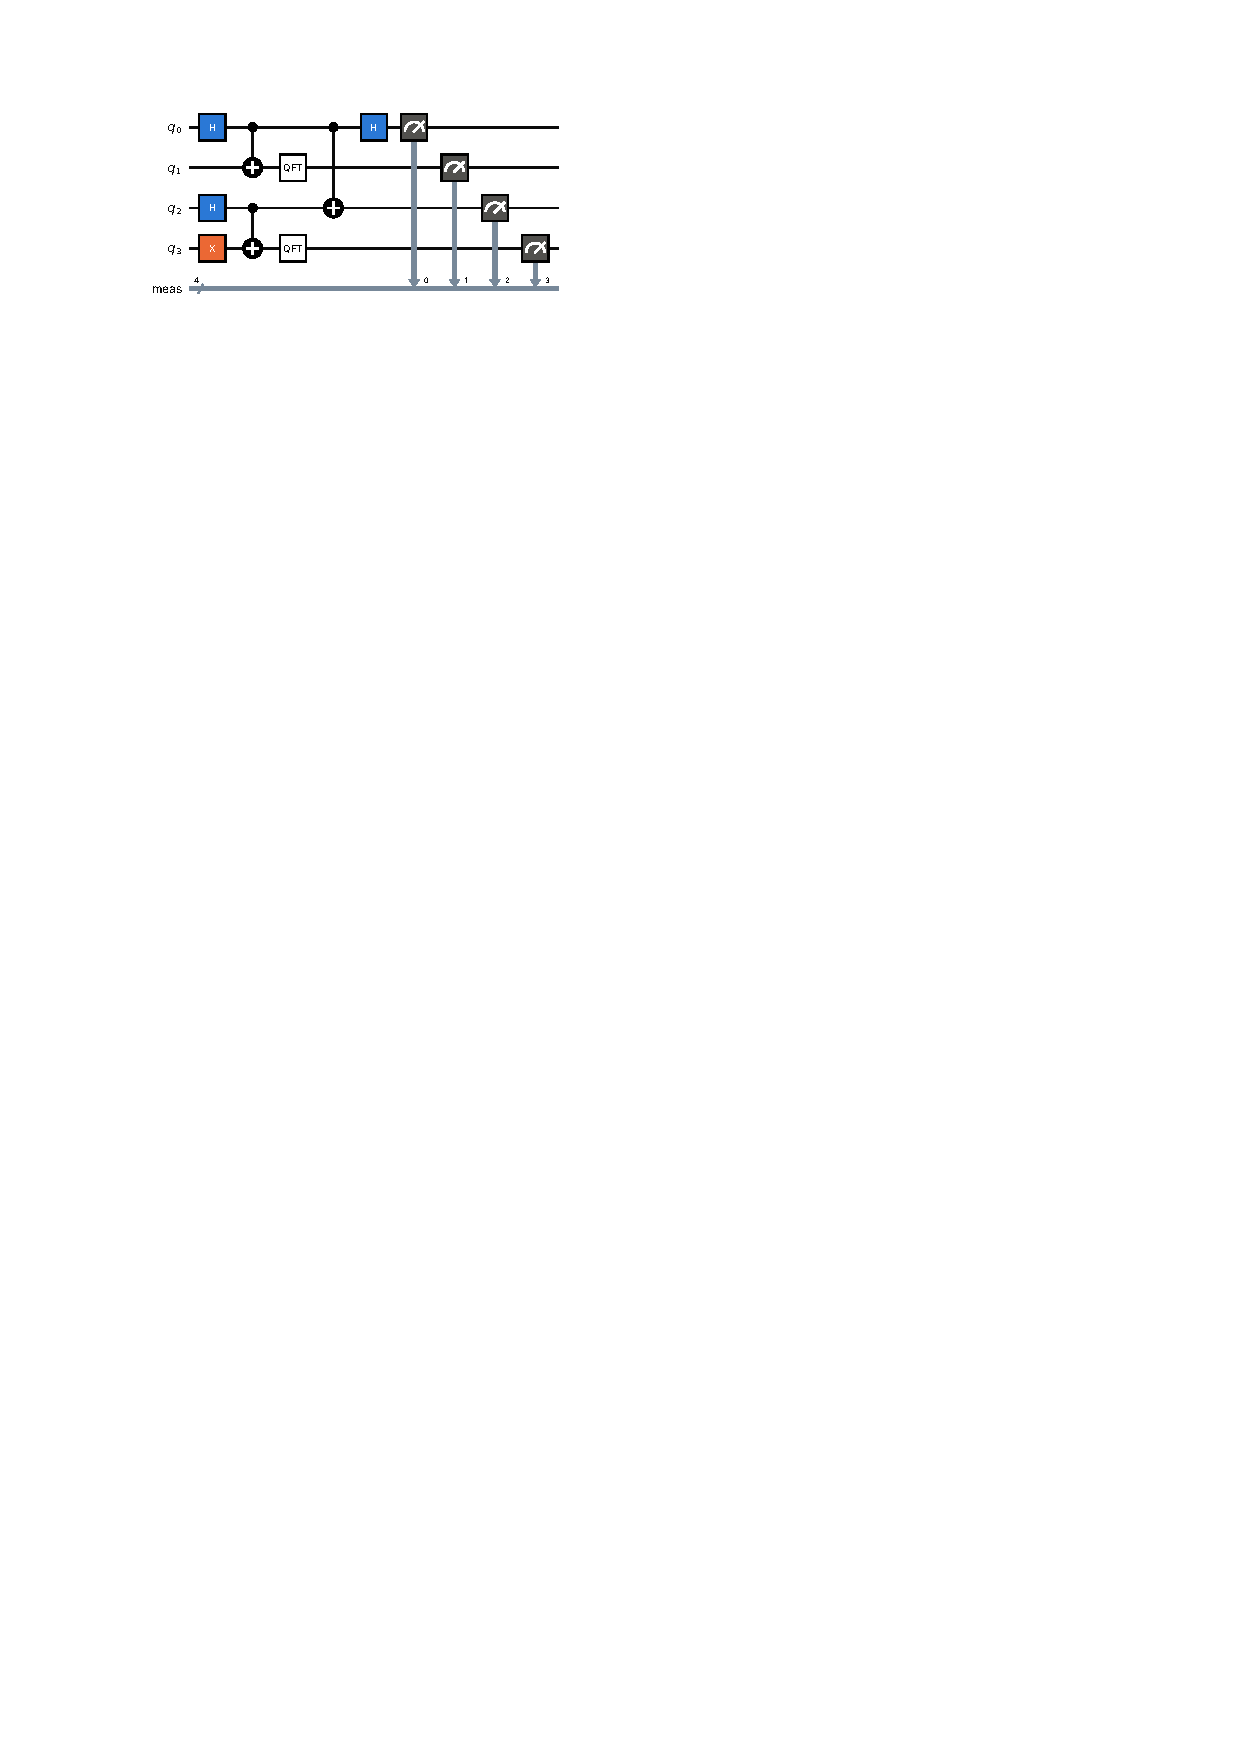
\includegraphics[width=\linewidth]{figs/quantique-1}
\caption{Circuit du test DCP pour $n = 1$, produit par
le code du projet. Les qubits $q_0$, $q_1$ et $q_2$, $q_3$ portent deux
échantillons (ici $x_1 = 0$, $x_2 = 1$, $s = 1$). Après les QFT, la
porte CNOT relie les deux qubits de réflexion et la porte H
finale révèle la parité de $s$ sur $q_0$.}\label{f:circuit}
\end{figure}

\subsection{Le Protocole et sa Réussite Théorique}
Alice et Bob conviennent de $n$, du nombre d'essais $t$ et
du nombre de manches $r$. À chaque manche, Alice tire un
secret $s$ et envoie des paires d'échantillons. Bob dispose
de $t$ essais pour trouver la parité, et répond au hasard s'il
n'y parvient pas. Alice compare enfin la proportion de
bonnes réponses à la valeur attendue. Un joueur classique
qui répond au hasard obtient 50~\%.

Pour deux échantillons, la probabilité de ne pas obtenir
de collision vaut $k = 1 - 1/N$, et un essai réussit avec
probabilité $(1-k)/2 = 1/(2N)$. Lin et Wen en déduisent
la réussite d'un appareil sans bruit~\cite{linwen} :
\begin{equation}\label{e:p}
p(t) = 1 - \frac12\left(1 - \frac{1}{2N}\right)^{t}.
\end{equation}
Pour $n = 1$ et $t = 15$, $p = 0{,}993$. Dans la suite, nous
rapportons plutôt la proportion de manches où Bob
trouve la bonne parité sans recourir au hasard, notée
$p_0(t) = 1 - (1 - 1/(2N))^t$. C'est la quantité mesurée sur
la machine, et elle sépare plus nettement un appareil
quantique d'un joueur classique.

\section{Implémentation}\label{s:impl}
\pa{Préparation des échantillons.} Pour chaque paire
$(x,\, x + s \bmod N)$, le code écrit les bits des deux valeurs
sur le registre : un bit qui vaut 1 dans les deux branches
donne une porte X, un bit qui ne vaut 1 que dans la
seconde donne une porte CNOT contrôlée par le qubit
de réflexion, et un bit qui ne vaut 1 que dans la première
donne les deux. Le qubit de réflexion est d'abord placé
en superposition par une porte de Hadamard.

\pa{Résolution.} La QFT de la bibliothèque Qiskit est
appliquée à chaque registre, puis la porte CNOT et la
porte H finale sont ajoutées avant la mesure de tous les
qubits. Un essai correspond à un seul tir (\en{shot}) du circuit.

\pa{Exécution.} En simulation, le code utilise le simulateur
Aer. Sur machine, il ouvre une session Qiskit Runtime sur
le processeur IBM le moins chargé, transpile les circuits
avec le gestionnaire de passes prédéfini, et envoie les $t$
essais d'une manche en un seul lot de circuits à un tir.
Les manches non résolues ne sont pas complétées par
une réponse au hasard. Le passage du simulateur à la
machine a demandé de traiter le placement des qubits
logiques sur la topologie du processeur : les portes SWAP
ajoutées par le transpileur rapprochent les qubits qui
doivent interagir, au prix de bruit supplémentaire.

\pa{Reproduction.} Toutes les simulations de ce rapport
ont été relancées avec le code du projet, sur 1\,000 manches
par point pour $n = 1$ et 500 pour $n = 2$. Le bruit d'un
processeur réel est reproduit avec le modèle de bruit du
processeur IBM Manila à cinq qubits, construit à partir
des données de calibration conservées dans Qiskit. C'est
sur ce processeur que Lin et Wen ont mené leur propre
expérience à quatre qubits.

\begin{figure}[t]
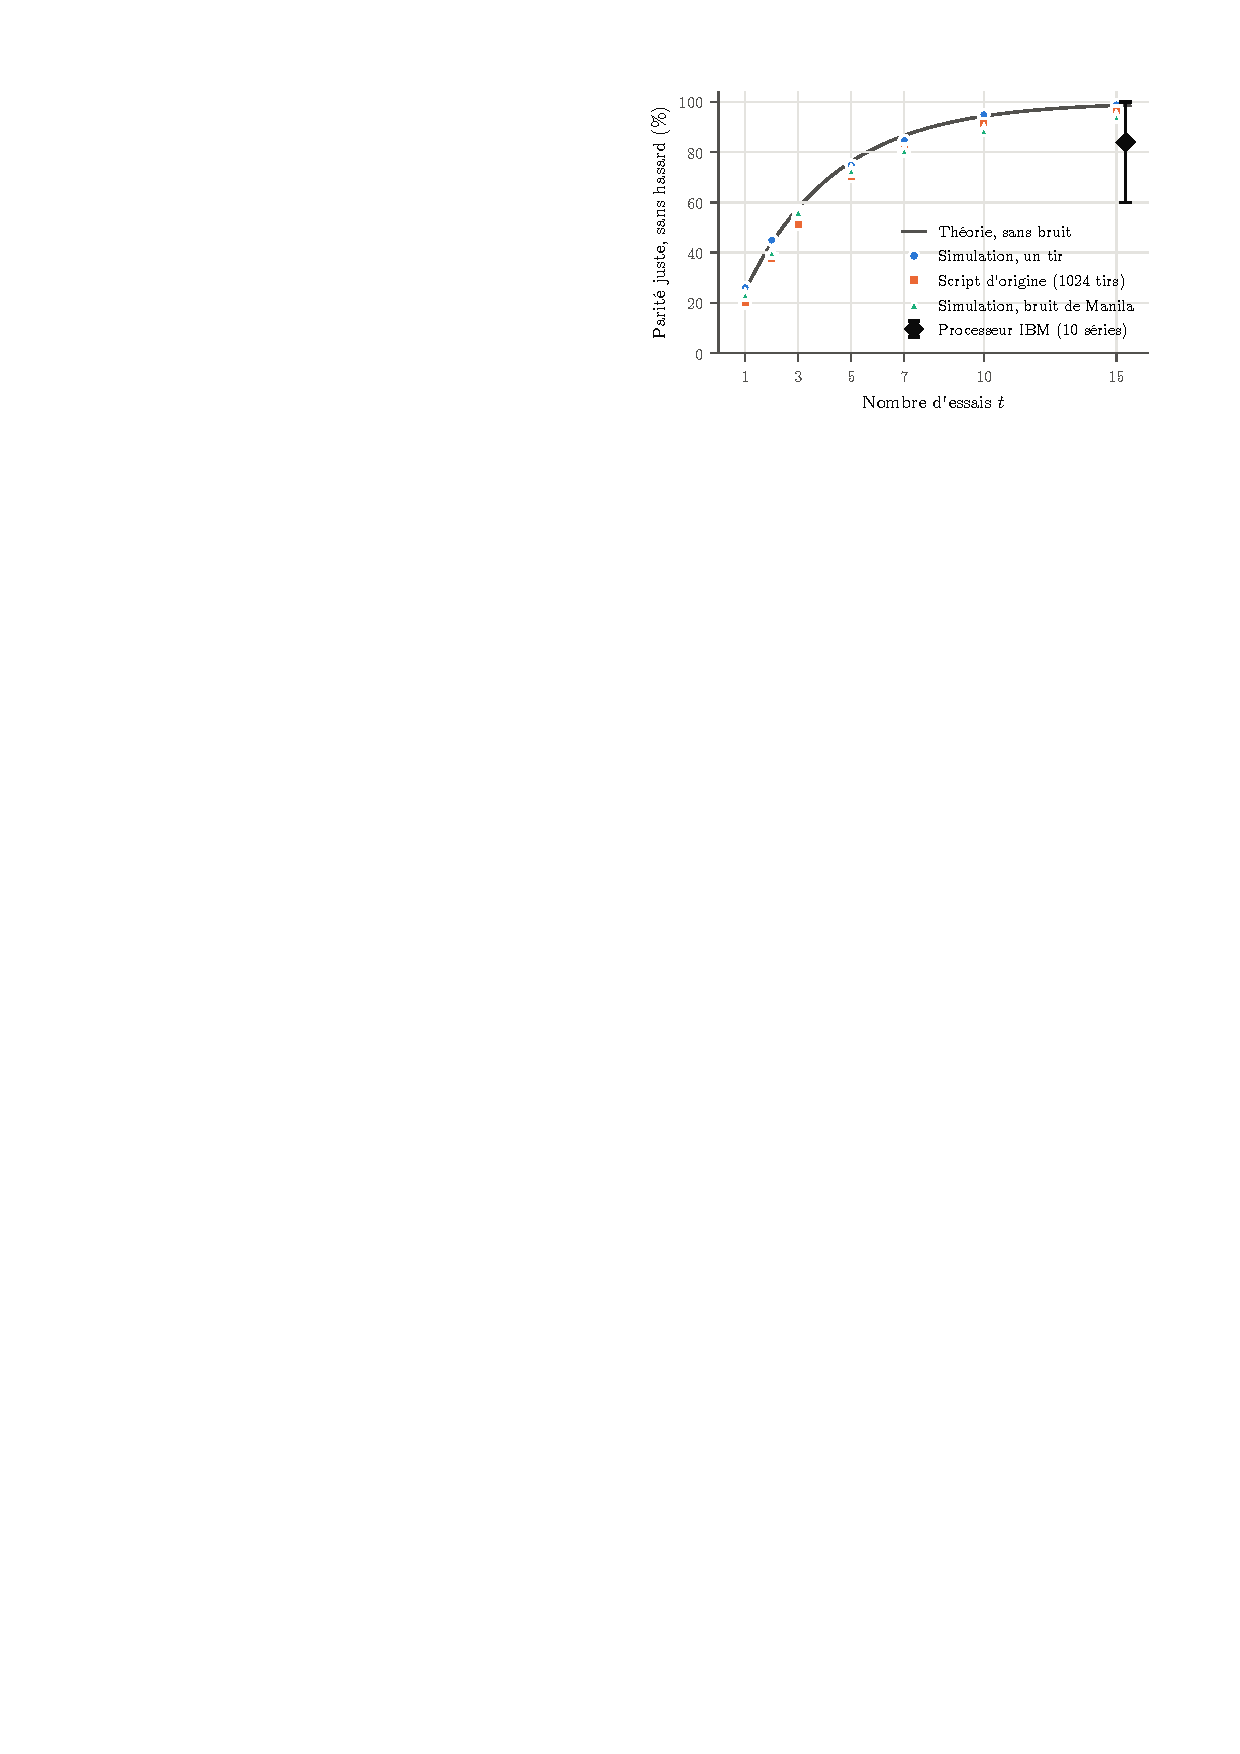
\includegraphics[width=\linewidth]{figs/quantique-2}
\caption{Proportion de manches où Bob trouve la bonne
parité sans répondre au hasard, pour $n = 1$, selon le nombre
d'essais $t$. La courbe pleine est la valeur théorique $p_0(t)$. Les
points sont des simulations sur 1\,000 manches ; le losange est
la mesure sur processeur IBM, avec l'étendue de ses dix séries.}\label{f:n1}
\end{figure}

\section{Résultats pour $n = 1$}\label{s:n1}
\pa{Simulation sans bruit.} Avec un tir par essai, la simulation suit la courbe théorique sur toute la plage de $t$
(figure~\ref{f:n1}). L'écart maximal, 2,0 points, est de l'ordre de la
fluctuation statistique attendue sur 1\,000 manches. Pour
$t = 15$, Bob trouve la parité dans 98,9~\% des manches,
contre 98,7~\% en théorie. Toutes les parités trouvées sont
justes, comme le prévoit l'analyse en l'absence de bruit.

\pa{Script de simulation d'origine.} Le premier script
de simulation du projet exécutait 1024 tirs par essai et
retenait le premier résultat du dictionnaire renvoyé par
le simulateur. Ce résultat n'est pas tiré uniformément
parmi les issues possibles, si bien que les manches résolues
sont sous-représentées : 20~\% pour $t = 1$ au lieu de 25~\%,
et 96,3~\% pour $t = 15$ au lieu de 98,7~\%. La version à un
tir, celle qu'exécute la machine, corrige ce biais.

\pa{Bruit simulé.} Avec le modèle de bruit du processeur
Manila, la parité trouvée n'est plus toujours juste. Pour
$t = 15$, Bob résout 98,9~\% des manches, mais sa parité
est fausse dans 4,9~\% d'entre elles, si bien qu'il ne répond
juste que dans 94,1~\% des manches. Le bruit perturbe
à la fois la détection des collisions et la phase $(-1)^s$
portée par le qubit de réflexion, deux effets que cette
seule mesure ne permet pas de séparer.

\pa{Processeur IBM.} Le protocole complet a été exécuté
pour $n = 1$ et $t = 15$, en dix séries de dix manches. Les
séries donnent 100, 100, 70, 100, 60, 100, 70, 70, 90 et
80~\% de bonnes réponses, soit 84~\% sur l'ensemble des 100
manches. Un joueur classique qui répondrait au hasard
aurait une probabilité de l'ordre de $10^{-12}$ d'atteindre
ce score. La machine fait donc nettement mieux que le
hasard, mais moins bien que le modèle de bruit de Manila
(94,1~\%). L'écart dépasse la seule fluctuation statistique.
Il peut venir d'un processeur plus bruité que Manila, ou
du placement des qubits choisi par le transpileur, dont
les portes SWAP ajoutent des erreurs.

\begin{figure}[t]
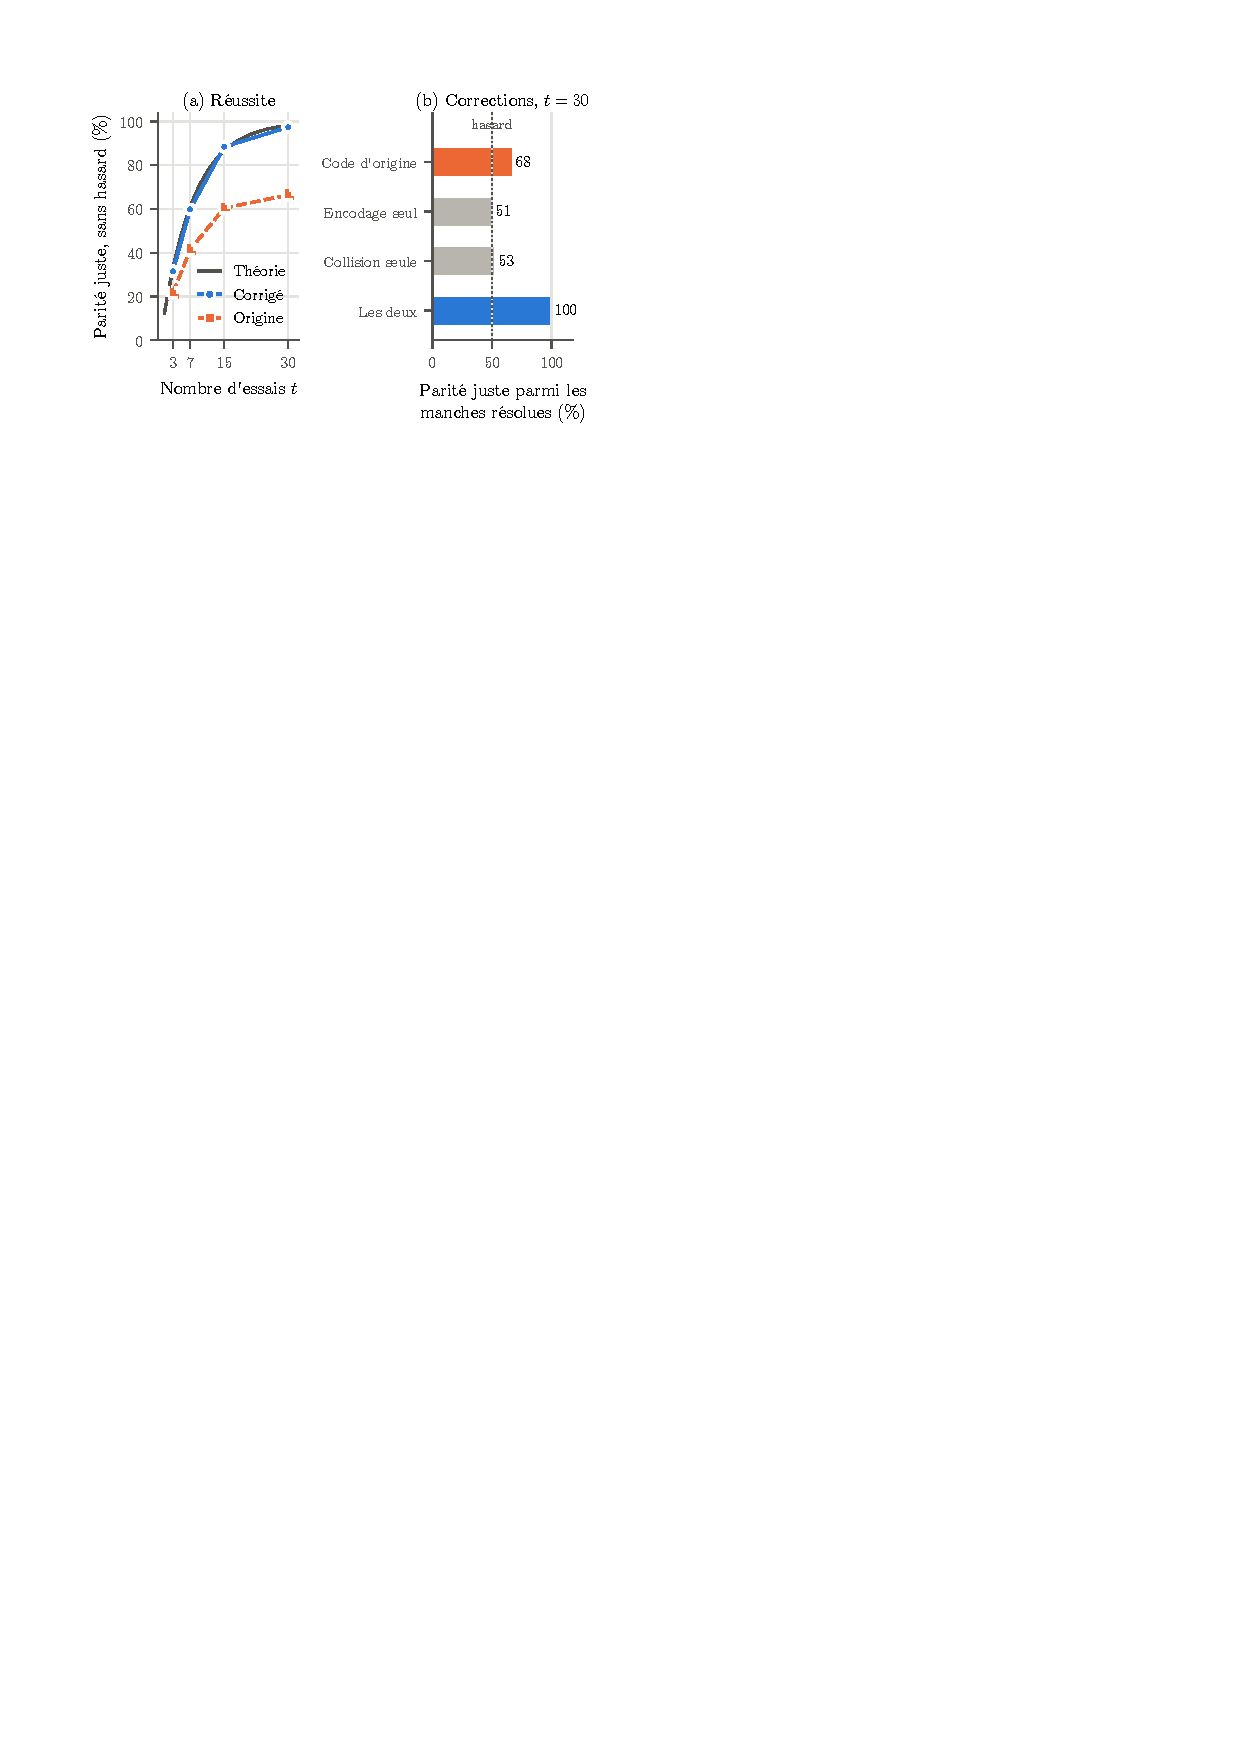
\includegraphics[width=\linewidth]{figs/quantique-3}
\caption{Simulation sans bruit pour $n = 2$, sur 500 manches
par point. (a) Proportion de manches où la parité est retrouvée
sans hasard, pour le code d'origine et la version corrigée, face
à la théorie. (b) Part des manches résolues dont la parité est
juste, pour $t = 30$, selon les corrections appliquées.}\label{f:n2}
\end{figure}

\section{Le Cas $n \geq 2$ : une Question d'Ordre des Bits}\label{s:n2}
Pour $n = 2$, les résultats du projet restaient entre 52~\%
et 61~\%, loin de la théorie. Une relecture du code en
explique la raison. Deux conventions d'ordre des bits se croisaient :
\begin{itemize}
\item la fonction de préparation écrit les entiers $x$ et $x + s$ poids fort en premier sur les qubits du registre,
alors que la QFT de Qiskit considère le premier qubit comme le bit de poids faible ;
\item le test de collision compare les bits de poids faible des
deux mesures, alors que ParitySolve exige que ce soit le bit de poids fort qui diffère.
\end{itemize}
Pour $n = 1$, le registre ne compte qu'un qubit et les deux
conventions coïncident, ce qui explique que le problème soit passé inaperçu.

Le code d'origine résout bien les manches (figure~\ref{f:n2}a),
mais la parité obtenue n'est juste que dans 68~\% des
manches résolues pour $t = 30$ (figure~\ref{f:n2}b). Les deux erreurs
se compensent en partie : corriger seulement l'encodage
ou seulement le test de collision ramène la parité juste à
51~\% et 53~\%, soit le hasard. En corrigeant les deux, la
parité est juste dans 100~\% des manches résolues, et la
proportion de bonnes réponses suit la théorie, de 32~\%
pour $t = 3$ à 97~\% pour $t = 30$, contre 33~\% et 98~\% attendus.

\section{\en{Key Leasing} sur Canal Classique}\label{s:kl}
\subsection{Principe}
Le \en{key leasing} permet à un client de prêter une clé
de déchiffrement quantique à un serveur, puis d'obtenir
la preuve que cette clé a été détruite~\cite{chardouvelis,phan}. Tout passe par un canal classique :
\begin{itemize}
\item le client génère une paire de \en{noisy trapdoor claw-free functions}
(NTCF), construites sur LWE, et publie la partie publique ;
\item le serveur prépare un \en{claw state} $\tfrac{1}{\sqrt 2}(\ket{0}\ket{x_0} + \ket{1}\ket{x_1})$,
superposition de deux antécédents d'une même image, qui sert de clé de déchiffrement ;
\item pour rendre la clé, le serveur la mesure dans la base de
Hadamard et renvoie le résultat, que le client vérifie grâce à sa \en{trapdoor}.
\end{itemize}
Un \en{claw state} a exactement la forme d'un échantillon
DCP, avec $x_1 - x_0$ dans le rôle du secret. L'idée du projet
était donc de produire les échantillons du test DCP par
le \en{key leasing}, ce qui supprime le besoin d'un canal quantique.

\subsection{Synthèse du \en{Claw State}}
Le code construit l'état $\sum_{b,x} \ket{b}\ket{x}\ket{f'_k(b,x)}$ à partir
de la table de vérité de $f'_k(b,x) = A\,x + b\,t \bmod q$, où
$(A, t)$ est la clé publique. Pour chaque ligne de la table
qui produit un 1, des portes X sélectionnent l'entrée et
une porte de Toffoli inscrit le bit de sortie. La mesure du
registre de sortie projette alors $(b, x)$ sur les antécédents
d'une même image, c'est-à-dire sur un \en{claw state}. Deux
de ces états sont ensuite passés au circuit ParitySolve.

\begin{table}[t]
\caption{Préparation de deux échantillons pour $n = 1$ :
nombre de portes avant mesure, en portes de haut niveau
puis après décomposition sur la base d'IBM, en moyenne sur 40 tirages.}\label{t:portes}
\centering\small
\begin{tabular}{lcc}
\toprule
Préparation & Haut niveau & Base IBM\\
\midrule
Directe (test DCP) & 4 & 8\\
\en{Key leasing} & 10 & 72\\
\bottomrule
\end{tabular}
\end{table}

\subsection{Résultats et Limites}
La chaîne fonctionne de bout en bout : génération des
clés, synthèse des \en{claw states} et test DCP. Le coût est
nettement plus élevé, puisque chaque porte de Toffoli se
décompose en six CNOT et plusieurs rotations. Il faut
en moyenne 72 portes pour préparer deux échantillons,
contre 8 pour la préparation directe (tableau~\ref{t:portes}).

Les paramètres utilisés sont des paramètres jouets,
$q = 2$ et $n = 1$, pour tenir dans quelques qubits. Avec la
matrice publique $A = 2$, le terme $A\,x$ s'annule modulo 2
et $f'_k(b,x) = b\,t$ ne dépend plus de $x$. Mesurer la sortie
fixe alors $b$, ou laisse $x$ indépendant de $b$, et l'état obtenu
ne porte plus de secret. Le secret du test DCP n'intervient
d'ailleurs pas dans la préparation. La réussite attendue
est donc exactement 50~\%. Les huit exécutions du script
du projet, de 50 manches chacune avec $t = 30$, donnent
de 36~\% à 60~\%, soit 50~\% en moyenne, ce qui est bien le
niveau du hasard. Les 60~\% observés pendant le projet
relevaient donc de la fluctuation statistique.

Pour que le \en{key leasing} produise de vrais échantillons, il faut des paramètres LWE pour lesquels $f'$ reste
injective et difficile à inverser. Le module $q$ et la dimension
$n$ grandissent alors, et le nombre de qubits et de portes
de Toffoli dépasse ce que les machines actuelles exécutent
avec une fidélité suffisante. Les travaux de Phan et al.~\cite{phan},
qui ramènent le module à une taille polynomiale, vont
dans le sens d'une telle mise en œuvre.

\section{Discussion et Limites}\label{s:disc}
\pa{La taille de l'échantillon.} La mesure sur machine
repose sur 100 manches. Elle suffit à écarter le hasard,
mais pas à mesurer finement la qualité du processeur :
d'une série de dix manches à l'autre, la réussite varie de
60~\% à 100~\%. Le processeur était choisi automatiquement
comme le moins chargé, et ses données de calibration
n'ont pas été conservées, ce qui empêche une comparaison
directe avec le modèle de bruit.

\pa{La triche.} Lin et Wen identifient deux façons de dépasser la réussite attendue avec moins de qubits : profiter
d'un long temps de relaxation pour remplacer un seul
échantillon à la fois, ou déplacer les qubits de réflexion
par des portes SWAP~\cite{linwen}. Imposer un délai entre les essais, plus long que le temps de relaxation des machines
actuelles, neutralise ces deux stratégies.

\pa{Les conventions de Qiskit.} Le défaut décrit en section~\ref{s:n2} tient à la convention \en{little-endian} de Qiskit, où
le premier qubit d'un registre porte le bit de poids faible
et où les chaînes de mesure se lisent du dernier qubit au
premier. Ce type d'erreur reste invisible quand $n = 1$. Un
test systématique pour $n \geq 2$ contre la formule~\eqref{e:p}, en
simulation sans bruit, l'aurait détecté immédiatement.

\pa{Perspectives.} Le test DCP peut servir d'étalon pour
comparer des processeurs, en mesurant la réussite $p_0(t)$
pour un même jeu de paramètres. Avec la correction
de la section~\ref{s:n2}, des exécutions sur machine pour $n = 2$
et $n = 3$ deviennent pertinentes. Il resterait aussi à
mesurer expérimentalement la probabilité de collision,
pour séparer l'effet du bruit sur les collisions de son effet sur la phase.

\section{Conclusion}
Ce projet a implémenté en Qiskit le test de quanticité
DCP de Lin et Wen et l'a exécuté sur un processeur
d'IBM. Pour $n = 1$, la simulation reproduit la théorie
et la machine retrouve la parité du secret dans 84~\% des
cas, un score hors de portée d'un joueur classique. La
relecture du code pour $n \geq 2$ a mis en évidence une
incohérence d'ordre des bits, dont la correction rétablit l'accord avec la théorie.

Le \en{key leasing} sur canal classique a été implémenté jusqu'au bout de la chaîne, de la clé publique au test
DCP. Il montre surtout l'écart entre ces protocoles et
les machines actuelles : avec des paramètres assez petits
pour être exécutés, les états produits ne portent plus
de secret. Ce constat rejoint la motivation des travaux
récents qui cherchent à réduire la taille des paramètres LWE nécessaires.

{\small
\begin{thebibliography}{9}\setlength{\itemsep}{1pt}
\bibitem{linwen} R. Lin et W. Wen, «~A Quantum Computation Capability Verification Protocol for NISQ Devices with Dihedral Coset Problem~», arXiv:2202.06984, 2022.
\bibitem{phan} D. H. Phan, W. Wen, X. Yan et J. Zheng, «~Adaptive Hardcore Bit and Quantum Key Leasing over Classical Channel from LWE with Polynomial Modulus~», \emph{ASIACRYPT}, 2024.
\bibitem{chardouvelis} O. Chardouvelis, V. Goyal, A. Jain et J. Liu, «~Quantum Key Leasing for PKE and FHE with a Classical Lessor~», \emph{IACR Cryptology ePrint Archive}, 2023/1640, 2023.
\bibitem{brakerski} Z. Brakerski, P. Christiano, U. Mahadev, U. Vazirani et T. Vidick, «~A Cryptographic Test of Quantumness and Certifiable Randomness from a Single Quantum Device~», \emph{FOCS}, IEEE, 2018.
\bibitem{kuperberg} G. Kuperberg, «~A Subexponential-Time Quantum Algorithm for the Dihedral Hidden Subgroup Problem~», \emph{SIAM Journal on Computing}, vol.~35, n\textsuperscript{o}~1, pp.~170--188, 2005.
\bibitem{regev} O. Regev, «~Quantum Computation and Lattice Problems~», \emph{SIAM Journal on Computing}, vol.~33, n\textsuperscript{o}~3, pp.~738--760, 2004.
\bibitem{preskill} J. Preskill, «~Quantum Computing in the NISQ Era and Beyond~», \emph{Quantum}, vol.~2, p.~79, 2018.
\bibitem{qiskit} A. Javadi-Abhari et al., «~Quantum Computing with Qiskit~», arXiv:2405.08810, 2024.
\end{thebibliography}}
\end{document}
